\section{Smith-Diagramm}

\subsection{Allgemein} \label{sec:Smith_All}


%$m$             : Anpassungsfaktor
%
%$s$             : inverser Anpassungsfaktor
%
%$\underline{r}$ : Reflexionsfaktor
%
%$1$             : Anpassungspunkt

\subsubsection{Normierte Impedanz}
gilt nur für \textbf{verlustlose} Leitung!
\begin{align*}
	\underline{z}_n= \frac{\underline{Z}(l)}{Z_L} &= \frac{\underline{Z}_2+jZ_L\cdot\tan(\beta l)}{Z_L+j\underline{Z}_2\cdot\tan(\beta l)}
	&= \frac{\frac{\underline{Z}_2}{Z_L}+j \tan(\beta l)}{1+j\frac{\underline{Z}_2}{Z_L}\cdot\tan(\beta l)}&
\end{align*}

allgemeine Gleichung \textbf{mit Verlusten} (siehe auch Kap. \ref{sec:Leitungen_allg_Gleichungen}.)\\
Ersetze: \quad $\tan \rightarrow \tanh$ und $\beta l \rightarrow \underline{\gamma} l$
\subsubsection{verlustloser Reflexionsfaktor}
%$ \underline{U}_r(l) = \underline{U}_r(l=0) \cdot e^{-j\beta l} \qquad \underline{U}_h(l) = \underline{U}_h(l=0) \cdot e^{j\beta l} $
Immer gültig, auch ohne Quelle!\\
$ \underline{r}(l) = \underline{r} \qquad \underline{r}_{(l=0)} = \underline{r}_2 \qquad 0<r<1 \qquad 0<\Psi<2\pi \, [\ang{360}] $\\

$L_n$: reale Leitungslänge von Last zu Eingang.
\begin{flalign*}
	\Aboxed{\underline{r}_n &= \underline{r}_2 \cdot e^{-j2\beta L_n}	
	= \underline{r}_2 \cdot e^{-j4\pi \frac{L_n}{\lambda}}}\\
%	 &= |\underline{r}_2| \cdot e^{-j\Psi_0} \cdot e^{-j(\beta L_n)} 
	 &= |\underline{r}_2| \cdot e^{j(\Psi_0-2\beta L_n)} & \Psi_0 (r_2) := \text{Startwinkel in \textbf{Radiant}}&\\
	 &=\frac{\underline{z}_n-1}{\underline{z}_n+1} \\
	\underline{r}_2 & = \frac{\underline{Z}_2-Z_L}{\underline{Z}_2+Z_L} = \frac{\underline{U}_2-\underline{I}_2Z_L}{\underline{U}_2 +\underline{I}_2 Z_L}
%\\
%\underline{z}_n & = \frac{1+\underline{r}}{1-\underline{r}}
\end{flalign*}
%    \begin{align*}
%        \Aboxed{ \underline{z}'(l) = \frac{Z(l)}{Z_L} = \frac{Z_2+jZ_L\cdot\tan(\beta l)}{Z_L+jZ_2\cdot\tan(\beta l)}} \\
%        \text{mit} \beta = \frac{2\pi}{\lambda}                                                \\
%        \text{auch ohne Quelle gültig!}
%    \end{align*}

\subsubsection{Schema und Kenngrößen}
\begin{center}
	

\usetikzlibrary{decorations.pathmorphing}
\usetikzlibrary{decorations.text}
\tikzset{
cross/.style={cross out, draw=black, minimum size=2*(#1-\pgflinewidth), inner sep=0pt, outer sep=0pt},
%     %default radius will be 1pt. 
cross/.default={3.5pt}
dot/.style={circle, fill=#1, inner sep=0, minimum size=4pt},
mini dot/.style={circle, inner sep=0pt, minimum size=2pt, pos=1, fill, node contents={}},
}

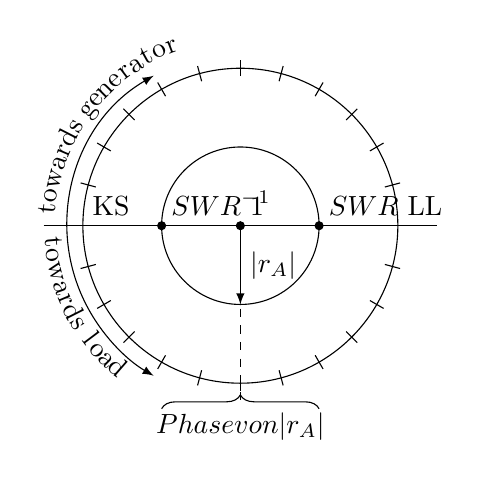
\begin{tikzpicture}
    \draw[-latex](0,0)--(0,-1) node[right, midway]{$|r_A|$};
    \draw[dashed](0,0)--(0,-2.25) node[below]{$\text{Phase von }|r_A|$};
    \draw [black,
        decorate,
        decoration = {brace,
                raise=5pt,
                amplitude=5pt}] (-1,-2.5) --  (1,-2.5);

    \draw[-,fill=black!100] (-1,0) circle (0.05) node[above right]{$\text{\tiny{SWR}}^\text{\tiny{-1}}$};
    \draw[-,fill=black!100] (0,0) circle (0.05);
    \draw[-,fill=black!100] (1,0) circle (0.05) node[above right]{$\text{\tiny{SWR}}$};
    \node at (-2,0)[above right]{KS};
    \node at (0,0)[above right]{1};
    \node at (2,0)[above right]{LL};
    \path (0,0) coordinate (c);
    \draw[-](-2.5,0)--(2.5,0);
    \node[, rotate around={85:(c)}] at (0,2.47){t};
    \node[, rotate around={81:(c)}] at (0,2.44){o};
    \node[, rotate around={76:(c)}] at (0,2.43){w};
    \node[, rotate around={71:(c)}] at (0,2.43){a};
    \node[, rotate around={67:(c)}] at (0,2.43){r};
    \node[, rotate around={63:(c)}] at (0,2.48){d};
    \node[, rotate around={59:(c)}] at (0,2.43){s};

    \node[, rotate around={53:(c)}] at (0,2.39){g};
    \node[, rotate around={49:(c)}] at (0,2.43){e};
    \node[, rotate around={45:(c)}] at (0,2.43){n};
    \node[, rotate around={41:(c)}] at (0,2.43){e};
    \node[, rotate around={37:(c)}] at (0,2.43){r};
    \node[, rotate around={33:(c)}] at (0,2.43){a};
    \node[, rotate around={29:(c)}] at (0,2.47){t};
    \node[, rotate around={25:(c)}] at (0,2.44){o};
    \node[, rotate around={21:(c)}] at (0,2.43){r};

    \node[, rotate around={-85:(c)}] at (0,-2.38){t};
    \node[, rotate around={-81:(c)}] at (0,-2.42){o};
    \node[, rotate around={-76:(c)}] at (0,-2.42){w};
    \node[, rotate around={-71:(c)}] at (0,-2.42){a};
    \node[, rotate around={-67:(c)}] at (0,-2.42){r};
    \node[, rotate around={-63:(c)}] at (0,-2.38){d};
    \node[, rotate around={-59:(c)}] at (0,-2.42){s};

    \node[, rotate around={-53:(c)}] at (0,-2.37){l};
    \node[, rotate around={-49:(c)}] at (0,-2.42){o};
    \node[, rotate around={-45:(c)}] at (0,-2.42){a};
    \node[, rotate around={-41:(c)}] at (0,-2.37){d};

    \draw[-, rotate around={0:(c)}](1.9,0)--(2.1,0);
    \draw[-, rotate around={15:(c)}](1.9,0)--(2.1,0);
    \draw[-, rotate around={30:(c)}](1.9,0)--(2.1,0);
    \draw[-, rotate around={45:(c)}](1.9,0)--(2.1,0);
    \draw[-, rotate around={60:(c)}](1.9,0)--(2.1,0);
    \draw[-, rotate around={75:(c)}](1.9,0)--(2.1,0);
    \draw[-, rotate around={90:(c)}](1.9,0)--(2.1,0);
    \draw[-, rotate around={105:(c)}](1.9,0)--(2.1,0);
    \draw[-, rotate around={120:(c)}](1.9,0)--(2.1,0);
    \draw[-, rotate around={135:(c)}](1.9,0)--(2.1,0);
    \draw[-, rotate around={150:(c)}](1.9,0)--(2.1,0);
    \draw[-, rotate around={165:(c)}](1.9,0)--(2.1,0);
    \draw[-, rotate around={180:(c)}](1.9,0)--(2.1,0);
    \draw[-, rotate around={195:(c)}](1.9,0)--(2.1,0);
    \draw[-, rotate around={210:(c)}](1.9,0)--(2.1,0);
    \draw[-, rotate around={225:(c)}](1.9,0)--(2.1,0);
    \draw[-, rotate around={240:(c)}](1.9,0)--(2.1,0);
    \draw[-, rotate around={255:(c)}](1.9,0)--(2.1,0);
    \draw[-, rotate around={270:(c)}](1.9,0)--(2.1,0);
    \draw[-, rotate around={285:(c)}](1.9,0)--(2.1,0);
    \draw[-, rotate around={300:(c)}](1.9,0)--(2.1,0);
    \draw[-, rotate around={315:(c)}](1.9,0)--(2.1,0);
    \draw[-, rotate around={330:(c)}](1.9,0)--(2.1,0);
    \draw[-, rotate around={345:(c)}](1.9,0)--(2.1,0);
    \draw[-](0,0) circle (1);
    \draw[-](0,0) circle (2);
    \draw[latex-latex](120:2.2) arc (120:240:2.2);

\end{tikzpicture}

\end{center}
Werte von Anpassungsfaktor $ m \rightarrow$ Werte von $ \Re{\underline{z}_n}: 0 \leq m \leq1 $
\begin{align*}
	m =\frac{1-|\underline{r}|}{1+|\underline{r}|} = \frac{U_{min}}{U_{max}} = \frac{I_{min}}{I_{max}} \qquad  |\underline{r}| = \frac{1-m}{1+m} \qquad \text{SWR}=\frac{1}{m}
\end{align*}
\begin{align*}
    \underline{z}_n & = \frac{\underline{Z}_n}{Z_L} = \frac{1+\underline{r}(l)}{1-\underline{r}(l)} \qquad \qquad |\underline{r}(l)|=\frac{\si{SWR}-1}{\si{SWR}+1} = \frac{1-m}{1+m}
    \\
    \underline{r}_n & = \frac{\underline{Z}_n-Z_L}{\underline{Z}_n+Z_L}= \frac{\underline{z}_n-1}{\underline{z}_n+1}    = \frac{1-\underline{y}_n}{1+\underline{y}_n} \\
%    m               & = \frac{1-|\underline{r}|}{1+|\underline{r}|}          \\
    \mathrm{SWR}               & = \frac{1}{m} = \frac{U_\text{max}}{U_\text{min}} = \frac{I_\text{max}}{I_\text{min}} = \frac{1+|r(l)|}{1-|r(l)|} = \frac{|U_h|+|U_r|}{|U_h|-|U_r|}= \dfrac{R_{\text{max}}}{Z_L}
\end{align*}




%\subsection{Zusammenschaltungen}
% \begin{center}
%     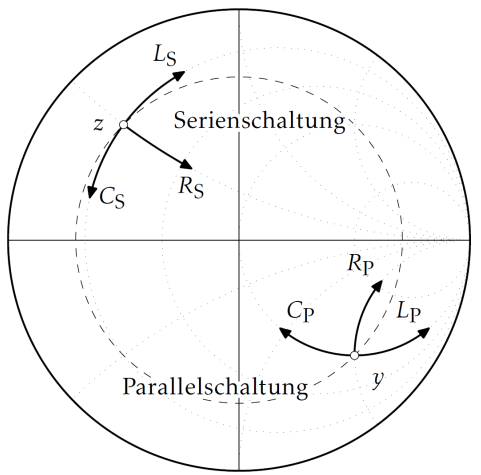
\includegraphics[width=.45\columnwidth]{Figures/Smithdiagramm_Zusammenschaltungen.png}
% \end{center}

%\columnbreak

\subsection{Maxima/Minima bei stehender Welle}\label{sec:max_min_stehende_welle}
Bei \textbf{verlustloser} Leitung:
\begin{align*}
	&U_{\texttt{max}} = |U_h| \cdot (1+|r(l)|) & U_{\texttt{min}} = |U_h| \cdot (1-|r(l)|) &\\
	&I_{\texttt{max}} = \left | \frac{U_h}{Z_L} \right | \cdot (1+|r(l)|) & I_{\texttt{min}} = \left| \frac{U_h}{Z_L} \right | \cdot (1-|r(l)|) &
\end{align*}
Für \textbf{Spannungen}: Abstand von der Last $ z $: \quad $ n=0,1,2,3... $
\begin{align*}
	 &z_{\texttt{min}} = \frac{\lambda}{4\pi}(\theta_{rad}+(2n+1)\pi)&
	 z_{\texttt{max}} = \frac{\lambda}{4\pi} \cdot (\theta_{rad}+2n\pi)&\\
	 \Aboxed{&\text{\textbf{Minima} alle}\: \frac{\lambda}{2} \rightarrow \frac{l}{\lambda}=0.5} \Aboxed{&
	 	\text{\textbf{Maxima} alle}\: \frac{\lambda}{4} \rightarrow \frac{l}{\lambda}=0.25} &
\end{align*}
$ \rightarrow $ Schnittpunkte mit der reellen Achse!\\
Strommaxima sind an Spannungsminima und umgekehrt.

\subsection{Impedanz/Admittanz umrechnen}
Spiegelung von $ \underline{z}_n $ um Mittelpunkt ergibt $ \underline{y}_n $.  (Phase $\pm 180^{\circ}$/$\pm \pi$)

\subsection[Von Last zu Quelle]{Lastseite $\rightarrow$ Quelle}
\begin{enumerate}
    \item $Z_L = Z_B$ ins Diagramm einzeichnen
    \item Lastimpedanz bestimmen,
          wenn z.B. Parallelschaltung etc.
    \item Normieren
          \[\underline{z}_n = \frac{\underline{Z}(l)}{Z_L} \]
    \item Im Chart eintragen
    \item Linie vom Mittelpunkt durch $\underline{z}_ns$ nach außen

          Ablesen und Notieren:

          $\rightarrow$ Relative Länge $\left[\frac{l}{\lambda}\right]$

          $\rightarrow$ Relativer Winkel in \textbf{Degree}
    \item Kreis einzeichen

          Ablesen und Notieren:

          $\rightarrow$ \textbf{Maxima}: rechter Schnittpunkt mit Re-Achse

          $\rightarrow$ \textbf{Minima}: linker Schnittpunkt mit Re-Achse

          $\rightarrow$ $ \underline{r} $ abmessen und aus oberer Skala auslesen
    \item Um Leitungslänge im UZS laufen
          $\rightarrow$ Linie vom Mittelpunkt durch neuen Punkt nach außen

          Ablesen und Notieren:

          $\rightarrow$Relativer Winkel
    \item Wenn $\alpha\neq 0$

          $\rightarrow$ Dämpung ausrechen
          $\rightarrow$ Um Faktor nach innen Spiralieren

    \item Dieser Punkt ist $\underline{z}_e$
    \item Eingangsimpedanz ablesen
          \[\underline{Z}_E = \underline{z}_e \cdot Z_L\]
\end{enumerate}


\usetikzlibrary{decorations.pathmorphing}
\usetikzlibrary{decorations.text}
\tikzset{
cross/.style={cross out, draw=black, minimum size=2*(#1-\pgflinewidth), inner sep=0pt, outer sep=0pt},
%     %default radius will be 1pt. 
cross/.default={3.5pt}
dot/.style={circle, fill=#1, inner sep=0, minimum size=4pt},
mini dot/.style={circle, inner sep=0pt, minimum size=2pt, pos=1, fill, node contents={}},
}
\begin{center}
 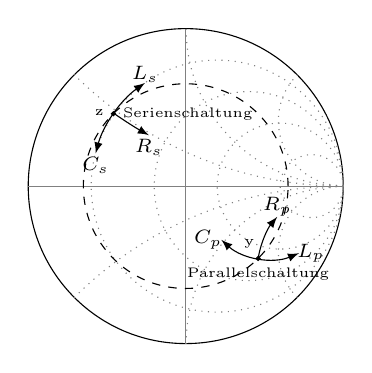
\begin{tikzpicture}    
    
    %Außenkreis
    \draw[-](0,0) circle (2);

    %Realteil Linien
    \draw[-, black!50](-2,0)--(2,0);

    \draw[dotted, black!50](0.4,0) circle (1.6);
    \draw[dotted, black!50](0.8,0) circle (1.2);
    \draw[dotted, black!50](1.2,0) circle (0.8);
    \draw[dotted, black!50](1.6,0) circle (0.4); 

    
    %Imaginärteil Linien
    \draw[-, black!50](0,-2)--(0,2);

    \draw[dotted, black!50, xshift = 13.25ex, yshift = -31.98ex](135:4.84)arc(135:90:4.84);
    \draw[dotted, black!50, xshift = 13.25ex, yshift = -13.25ex](180:2)   arc(180:90:2);
    \draw[dotted, black!50, xshift = 13.25ex, yshift = -5.485ex](225:.828)arc(225:90:.828);

    \draw[dotted, black!50, xshift = 13.25ex, yshift = 31.98ex](270:4.84)arc(270:225:4.84);
    \draw[dotted, black!50, xshift = 13.25ex, yshift = 13.25ex](270:2)   arc(270:180:2);
    \draw[dotted, black!50, xshift = 13.25ex, yshift = 5.485ex](270:.828)arc(270:135:.828);

    %Reflexionsfaktorkreis
    \draw[dashed](0,0) circle (1.3);

    %Serienschaltung
    \draw[-,fill=black!100] (-.919,.919) circle (0.025)node[left, yshift =.5] {\tiny z}node[right]{\tiny Serienschaltung};
    \draw[latex-latex, xshift = 2.65ex](125:1.6)node[above, yshift=-.75ex]{\scriptsize${L_s}$} arc (125:165:1.6)node[below, yshift=.5ex]{\scriptsize$C_s$};
    \draw[latex-, xshift = 13.25ex, yshift = 33.75ex](241:5.1)node[below, yshift=.5ex]{\scriptsize$R_s$}arc(241:235:5.1);

    %Parallelschaltung
    \draw[-,fill=black!100] (.919,-.919) circle (0.025)node[above left, xshift = .5ex]{\tiny y} node[below]{\tiny Parallelschaltung};
    \draw[-latex, xshift = 13.25ex, yshift = -7.25ex](170:1.1)arc(170:140:1.1)node[above, yshift=-.75ex]{\scriptsize$R_p$};

    \draw[latex-latex, xshift = 7.12ex](293:.925)node[right, xshift = -.95ex]{\scriptsize$L_p$}arc(293:227.5:.925)node[left, xshift = .85ex]{\scriptsize$C_p$};

\end{tikzpicture}
\end{center}

Positive/negative Blindwerte bewegen sich im/gegen den Uhrzeigersinn. Wirkwiderstände bewegen sich immer zum Leerlaufpunkt.

\subsection{Vorgehen mit geg. Eingangswiderstand}
Wenn mit dem Smith-Diagramm gearbeitet
wird, liefert dies die Schritte \ref{Ref L_anfang} und \ref{Bestimmen Z_E}
\begin{enumerate}
	\item Lastimpedanz
	\[ \underline{Z}_A = \dfrac{1}{\frac{1}{R_A} + j \omega C_A} \]
	\item Reflexion am Leitungsende
	\[ \underline{r}_A = \underline{r}(z=0) = \dfrac{Z_A - \underline{Z}_L}{Z_A + \underline{Z}_L} \]
	\item Reflexion am Leitungsanfang \label{Ref L_anfang}
	\[ \underline{r}_E = \underline{r}(z=d) =  \underline{r}_A \cdot e^{-j 2 \beta d}\]
	\item Bestimmung der Impedanz \label{Bestimmen Z_E}
	\[ \underline{Z}_E = \underline{Z}_L \cdot \dfrac{1 + \underline{r}_E}{1 - \underline{r}_E}\]
	\item Eingangswiderstand
	\[ \underline{Z}_E = \dfrac{1}{\frac{1}{\underline{Z}_E} + j \omega C_E}\]
\end{enumerate}

%\subsection{Reihen- und Parallelschaltung}
%Leitung transformiert den Abschluss
%\[ \underline{Z}_2 = R_2 + jX_2 \quad \text{bzw.} \quad \underline{Y}=G_2 + jB_2\]
%mit \[ \underline{Y}_2=\frac{1}{Z_2}  \]
%
%\subsubsection{ESB Serienschaltung}
%
%\[ P = \frac{\hat{I}^2_2 \cdot R_2}{2} \Rightarrow \hat{I}(l) = I^2_2 \cdot \sqrt{\frac{R_2}{R(l)}} \]